\documentclass[11pt,fleqn]{article}
\usepackage[a4paper, hmargin={2.8cm, 2.8cm}, vmargin={2.8cm, 2.8cm}]{geometry}  % Geometri-pakke: Styrer bl.a. maginer                              %
\usepackage[utf8]{inputenc}                                         % Lidt kodning så der ikke kommer problemer ved visse konverteringer            %
\usepackage[babel, lille, nat, da, farve]{ku-forside}               % KU-forside med logoer                                                         %
\def\HyperLinks{                                                    %  Hyperlinks-pakke, der laver referencer til links og tillader links til www   %
\usepackage[pdftitle={\TITEL},pdfauthor={\FORFATTER},               %  Der er foretaget et lille trick så pakken indlæses efter                     %
pdfsubject={\UNDERTITEL}, linkbordercolor={0.8 0.8 0.8}]{hyperref}} %  titlen defineres.                                                            %

\usepackage{lastpage}
\usepackage{fancyhdr}
\usepackage[toc]{appendix}
\usepackage{pdfpages}

\forfatter{Daniel Egeberg, Kristoffer Søholm og Sebastian Tørholm}
\dato{27 september, 2010}
\titel{Tredje opgave}
\undertitel{Menneske-datamaskine interaktion 2010}

\HyperLinks % Henter hyperlinks-pakke og sætter pdf-titel mm. til at svare til de just definerede

\pagestyle{fancy}
\lhead{{\small \FORFATTER}}
\chead{}
\rhead{}
\cfoot{\footnotesize Side \thepage \ af \pageref{LastPage}}

\setcounter{secnumdepth}{1}
\setcounter{tocdepth}{2}


\begin{document}

\maketitle

\tableofcontents


\thispagestyle{empty}

\section{Kontekstuel undersøgelse ved interview}

Vores interviewproces startede med at vi udarbejdede et script vi kunne følge. Vi valgte at følge en struktureret til semi-struktureret approach til at foretage de faktiske interview, hvor vi udeladte visse spørgsmål hvor det viste sig at være relevant.\footnote{Som set i Benyon 7.3}

Grundet tidsbegrænsning og manglende passende mennesker i vores omgangskreds var det desværre ikke muligt at ramme målgruppen præcist, så vi forsøgte at tilnærme det til bedste evne. Grundet dette var der måske nogle af interviewees'ne der ikke helt havde et lige så begrænset skill-set som en gennemsnitlig pensionist, hvilket kunne skjule visse problemområder.

Ydermere var det ikke muligt at mødes med alle folkene der skulle interviewest, så visse af interviews'ne blev fortaget over telefonen, hvorved vi mistede en del information vi kunne have fået ved at se hvordan de præcist reagerede og forsøgte at navigere på websiden.

Af personer har vi interviewet følgende:

\begin{description}
    \item[U1] {
    % Daniel
        En 63-årig efterlønsmodtager. Bruger computeren et par gange om ugen, primært til netbank, email og lidt informationssøgning. Bruger internettet et par timer om ugen. Det var ikke muligt at mødes med U1 for at foretaget et interview, så det blev foretaget over telefon.
    }
    \item[U2] {
    % Kristoffer
        En 70-årig pensionist, tidligere taxachauffør. Bruger primært computeren til et par google-søgninger, men printer også tilbud og spiller spil. Han bruger computeren ca. 8 timer om ugen.
    }
    \item[U3] {
    % Sebastian
    En 53-årig kvindelig læge. Bruger dagligt nettet til fx at checke mail, se røntgenbilleder osv.
    }
    \item[U4] {
    % Mathias
    En 70-årig pensionist. Meget aktiv mand, som bruger nettet meget, til blandt andet mails, blogs og nyheder.
    }
\end{description}

\subsection{Manuskript til interview}

Til interviewet fulgte vi følgende manuskript:

\begin{itemize}
    \item Grundlæggende information:
    \begin{itemize}
        \item Alder.
        \item Beskæftigelse? Hvis pensioneret, lavede personen før.
        \item Hyppighed af computerbrug.
        \item Antal timers internetbrug per uge.
        \item Hvad er vigtigt i forbindelse med brug af internettet?
        \item Har du brugt ældresagens hjemmeside før?
        \begin{itemize}
            \item Hvis ja: Kunne du forestille dig at bruge Ældre Sagens hjemmeside?
            \item Hvis nej: I hvilken forbindelse brugte du siden?
        \end{itemize}
        \item Hvad kunne være interessant for dig på sådan en side?
        \item Ældre Sagen tilbyder blandt andre ting rabatter på koncerter, hjælpemidler og lignende. Kunne du forestille dig at du ville bruge siden i den forbindelse?
        \item Hvilken information ville du ønske at se fremhævet i forbindelse med køb af følgende ting?
        \begin{itemize}
            \item Koncertbillet
            \item Høreapparat
            \item Ferierejse
            \item Cirkusbillet
            \item Social udflugt
        \end{itemize}
    \end{itemize}
    \item Test af Ældre Sagens hjemmeside:
    \begin{itemize}
        \item Hvad er din første indtryk af siden?
        \item Forestil dig at du gerne vil være medlem af Ældre Sagen. Prøv at finde information om at blive medlem.
        \begin{itemize}
            \item Vurdér oplevelsen på en skala fra 1--10, hvor 1 er meget nem og 10 er meget svær.
            \item Kommentarer?
        \end{itemize}
        \item Prøv at finde siden med medlemstilbud.
        \begin{itemize}
            \item Vurdér oplevelsen på en skala fra 1--10, hvor 1 er meget nem og 10 er meget svær.
            \item Kommentarer?
        \end{itemize}
        \item Du ønsker at købe en billet til musicalen ``Sværdet i Stenen''. Prøv at finde information om dette.
        \begin{itemize}
            \item Vurdér oplevelsen på en skala fra 1--10, hvor 1 er meget nem og 10 er meget svær.
            \item Kommentarer?
        \end{itemize}
        \item Hvordan var den generelle oplevelse af at bruge siden?
    \end{itemize}
    \item Test af Pensionistsagens prototypehjemmeside:
    \begin{itemize}
        \item Hvad er din første indtryk af siden?
        \item Forestil dig at du gerne vil være medlem af Ældre Sagen. Prøv at finde information om at blive medlem.
        \begin{itemize}
            \item Vurdér oplevelsen på en skala fra 1-10, hvor 1 er meget nem og 10 er meget svær.
            \item Kommentarer?
        \end{itemize}
        \item Prøv at finde siden med medlemstilbud.
        \begin{itemize}
            \item Vurdér oplevelsen på en skala fra 1-10, hvor 1 er meget nem og 10 er meget svær.
            \item Kommentarer?
        \end{itemize}
        \item Du ønsker at købe en billet til en. Prøv at finde information om dette.
        \begin{itemize}
            \item Vurdér oplevelsen på en skala fra 1-10, hvor 1 er meget nem og 10 er meget svær.
            \item Kommentarer?
        \end{itemize}
        \item Hvordan var den generelle oplevelse af at bruge siden?
    \end{itemize}
\end{itemize}

\section{Fortolkning af interview data}

Vi skabte vores affinitets-diagram ved at omforme vores interview-resultater til små, korte sætninger der dækkede et lille emne. Disse blev da fordelt ud på små sedler, som vi derefter arbejdede med at gruppere.
Generelt fandt vi ret god sammenhæng i mange af dem, men der var visse der ikke helt var relevante.

Vedlagt i bilag ses resultatet af vores affinitets-diagrammering, inklusiv overskrifter på vores grupperinger. Desuden kan man se billeder fra vores diagrammerings-proces.

Vi lagde mærke til følgende trends i vores resultater:

\begin{itemize}
    \item Vores ændring til menuen fik generelt positivt feedback, men dog var farverne ikke så populære.
    \item Menuerne er forvirrende, men dette vidste vi i forvejen.
    \item Information om accessibility og om pårørende kan tage med i forbindelse med arrangementer er vigtigt og bør highlightes.
    \item Teksten bør være større, med en klar overskrift så den ældre nemmere kan forstå hvor de er.
    \item Eksempelkategorierne er ikke altid helt logiske (fx at koncerter ikke er under underholdning).
    \item Søgefunktionaliteten er meget vigtig og bør forbedres.
    \item Arrangementer bør laves i samme stil som webshoppen for at skabe uniformitet; mange søgte derover for at finde information om koncerter.
    \item En let og gennemskuelig URL der er tilgivende kunne være godt.
\end{itemize}

\section{Alternative visioner}
Vi har fulgt visioneringsprocessen, som beskrevet i \cite[Kapitel 11]{Holtzblatt2005}, så tæt som muligt. Vi har ikke fulgt rollerne som beskrevet \cite[s. 214-216]{Holtzblatt2005}, da der så kun ville være 1 person til rent faktisk at fortælle historien. 


\subsection{Vision 1}
I vores første vision kom vi primært til at fokusere på en arrangementskalender samt dens betydning for resten af siden.
Vi udforskede kalenderens sammenhæng med både vores frontend (det som pensionisterne ser) og vores backend (det som pensionistsagens medarbejdere ser).
Derudover har vi forestillet os nogle nye features, f. eks. login med NemID, en personlig kalender til hver bruger og flere forskellige betalingsformer.

\subsubsection{Fordele}
\begin{itemize}
\item NemID kan gøre betaling nemt 
\item Kalenderen giver bedre overblik over arrangementer
\item Personlig kalender gør det muligt at huske hvilke arrangementer man skal til
\item Nye tilbud på forsiden kan give motivation til at vende tilbage oftere
\end{itemize}

\subsubsection{Ulemper}
\begin{itemize}
\item NemID gør det besværligt at logge ind
\item Visse betalingsformer kan være krævende at understøtte
\item Forsiden kan nemt blive for rodet
\item Personlig kalender kan nemt komme i vejen, hvis brugeren ikke bruger siden ofte
\end{itemize}

\subsection{Vision 2}
Her endte vi med at tage fat i selve webshop-delen af siden. Der er masser af features som de fleste moderne webshops har, f. eks. foreslåede varer ud fra tidligere søgninger og køb, produktanmeldelser, gavekort, produktsøgning osv. Desuden er der reklamer på forsiden, der promoverer interessante varer, eventuelt med tidsbegrænsede tilbud.

\subsubsection{Fordele}
\begin{itemize}
\item Andre brugeres anbefalinger i produktanmeldelser kunne gøre brugeren mere tryg ved køb
\item Gavekort kunne hjælpe på salget
\item Søgning gør det lettere at finde det man leder efter
\item Indlejrede videoer af produkterne i aktion kan motivere yderligere køb
\item Relaterede søgninger fra andre brugere kan inspirere brugere til at kigge på andre varer
\end{itemize}

\subsubsection{Ulemper}
\begin{itemize}
\item Brugere har en tendens til ikke at kigge på elementer, der ligner reklamer \cite{Grue}
\item For mange features kan gøre købsprocessen uoverskuelig
\item Relaterede søgninger virker ikke altid godt ved små udvalg af varer
\end{itemize}

\subsection{Konsolideret vision}
Ud fra evalueringen af de to foregående visioner har vi lavet en konsolideret vision. De to visioner overlapper ikke væsentligt, så det var muligt at sætte dem sammen uden at fjerne så meget. Vi droppede NemID, og alt efter hvor stor webshoppen er bliver relaterede søgninger formegentligt også droppet. Vi har også valgt store eventreklamer fra på forsiden for at holde den overskueligt, og i stedet valgt en liste over nye tilbud, som ligner indhold frem for reklamer.

\section{Detaljering af vision med storyboards}


\addcontentsline{toc}{section}{Litteratur}
\bibliographystyle{dk-plain}
\bibliography{references}

\renewcommand{\appendixtocname}{Bilag}
\renewcommand{\appendixpagename}{Bilag}
\begin{appendices}
    \section{Interview}
    \label{b:interview}
    \begin{itemize}
    \item Grundlæggende information:
    \begin{itemize}
        \item Alder.
        \item Beskæftigelse? Hvis pensioneret, lavede personen før.
        \item Hyppighed af computerbrug.
        \item Antal timers internetbrug per uge.
        \item Hvad er vigtigt i forbindelse med brug af internettet?
        \item Har du brugt ældresagens hjemmeside før?
        \begin{itemize}
            \item Hvis ja: Kunne du forestille dig at bruge Ældre Sagens hjemmeside?
            \item Hvis nej: I hvilken forbindelse brugte du siden?
        \end{itemize}
        \item Hvad kunne være interessant for dig på sådan en side?
        \item Ældre Sagen tilbyder blandt andre ting rabatter på koncerter, hjælpemidler og lignende. Kunne du forestille dig at du ville bruge siden i den forbindelse?
        \item Hvilken information ville du ønske at se fremhævet i forbindelse med køb af følgende ting?
        \begin{itemize}
            \item Koncertbillet
            \item Høreapparat
            \item Ferierejse
            \item Cirkusbillet
            \item Social udflugt
        \end{itemize}
    \end{itemize}
    \item Test af Ældre Sagens hjemmeside:
    \begin{itemize}
        \item Hvad er din første indtryk af siden?
        \item Forestil dig at du gerne vil være medlem af Ældre Sagen. Prøv at finde information om at blive medlem.
        \begin{itemize}
            \item Vurdér oplevelsen på en skala fra 1--10, hvor 1 er meget nem og 10 er meget svær.
            \item Kommentarer?
        \end{itemize}
        \item Prøv at finde siden med medlemstilbud.
        \begin{itemize}
            \item Vurdér oplevelsen på en skala fra 1--10, hvor 1 er meget nem og 10 er meget svær.
            \item Kommentarer?
        \end{itemize}
        \item Du ønsker at købe en billet til musicalen ``Sværdet i Stenen''. Prøv at finde information om dette.
        \begin{itemize}
            \item Vurdér oplevelsen på en skala fra 1--10, hvor 1 er meget nem og 10 er meget svær.
            \item Kommentarer?
        \end{itemize}
        \item Hvordan var den generelle oplevelse af at bruge siden?
    \end{itemize}
    \item Test af Pensionistsagens prototypehjemmeside:
    \begin{itemize}
        \item Hvad er din første indtryk af siden?
        \item Forestil dig at du gerne vil være medlem af Ældre Sagen. Prøv at finde information om at blive medlem.
        \begin{itemize}
            \item Vurdér oplevelsen på en skala fra 1-10, hvor 1 er meget nem og 10 er meget svær.
            \item Kommentarer?
        \end{itemize}
        \item Prøv at finde siden med medlemstilbud.
        \begin{itemize}
            \item Vurdér oplevelsen på en skala fra 1-10, hvor 1 er meget nem og 10 er meget svær.
            \item Kommentarer?
        \end{itemize}
        \item Du ønsker at købe en billet til en. Prøv at finde information om dette.
        \begin{itemize}
            \item Vurdér oplevelsen på en skala fra 1-10, hvor 1 er meget nem og 10 er meget svær.
            \item Kommentarer?
        \end{itemize}
        \item Hvordan var den generelle oplevelse af at bruge siden?
    \end{itemize}
\end{itemize}
    \section{Affinitetsdiagram}
    \label{b:aff}
    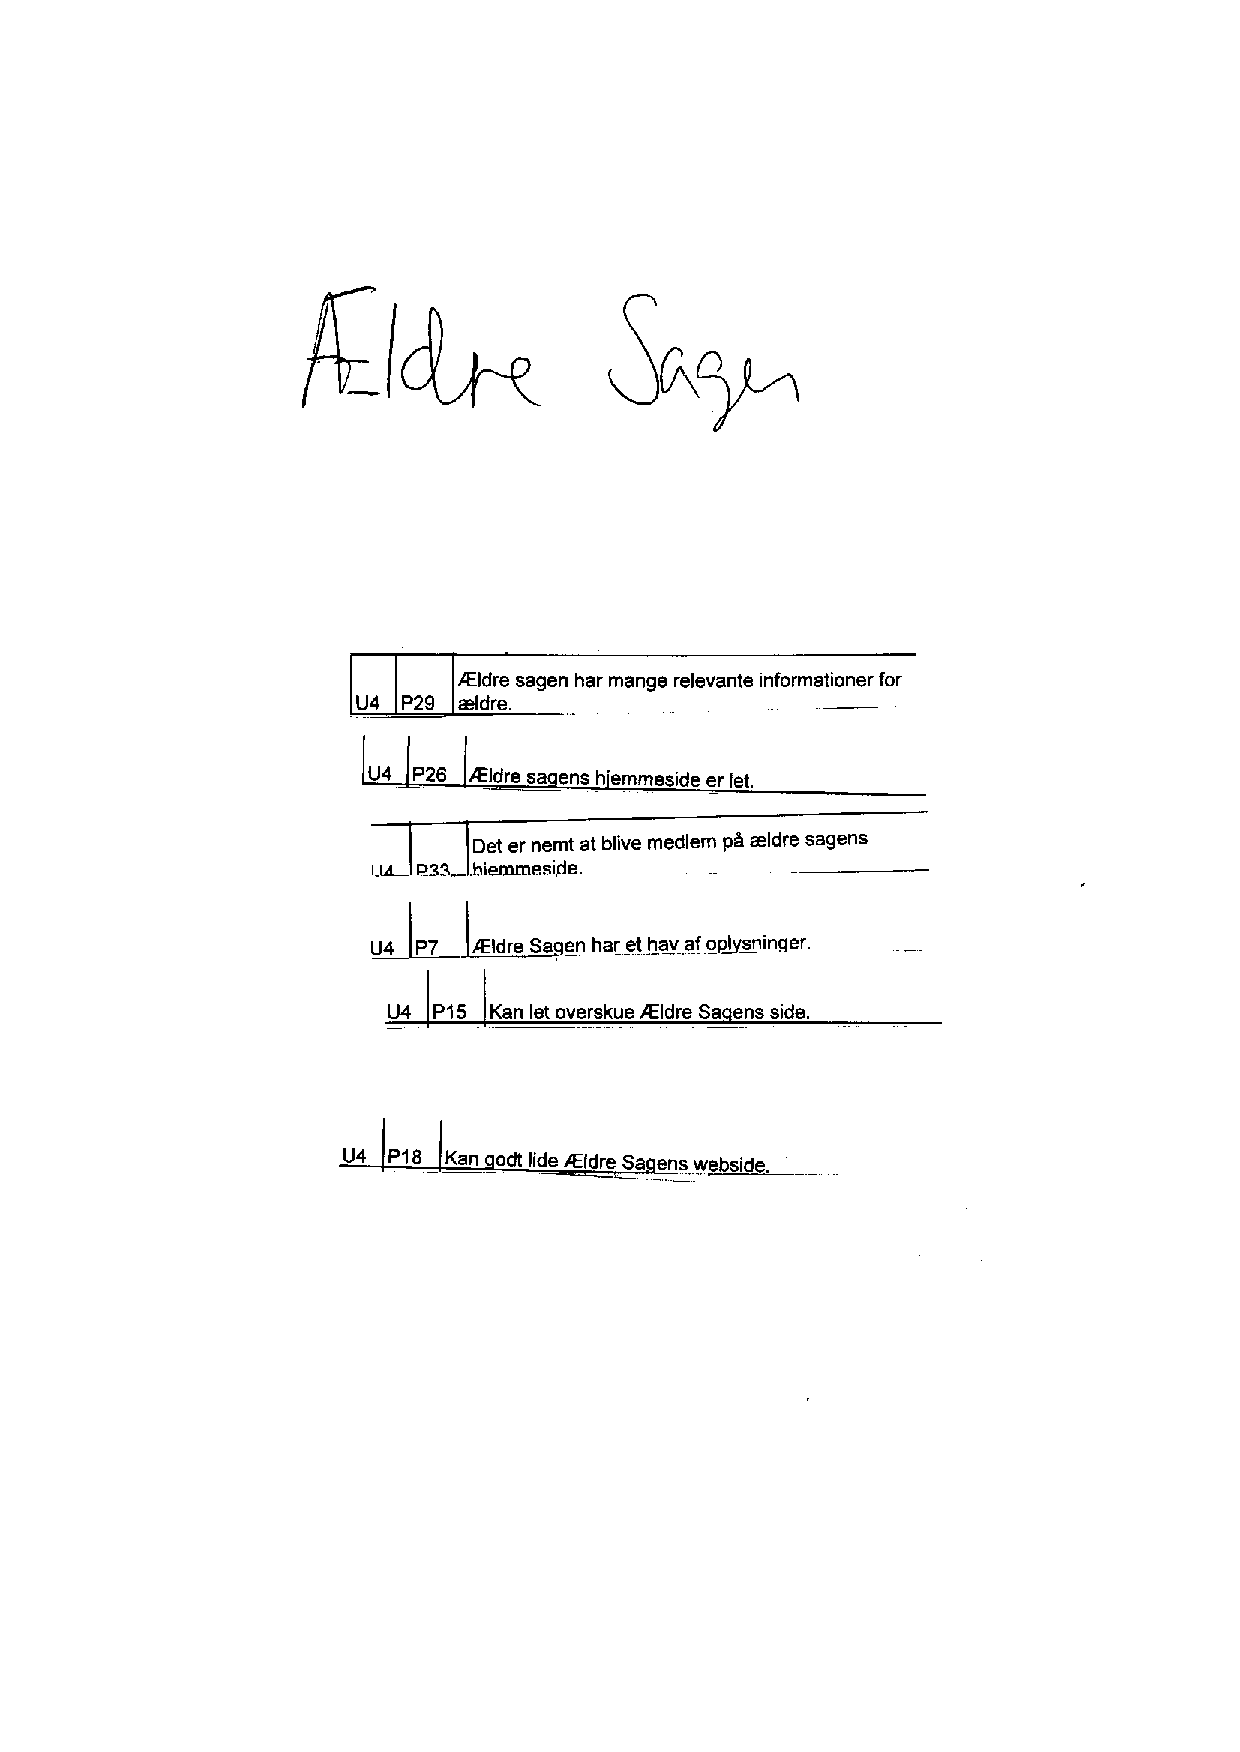
\includepdf[pages=-]{bilag_affinitet.pdf}

    \section{Arbejdet med affinitetsdiagrammering}
    \label{b:aff_billeder}
    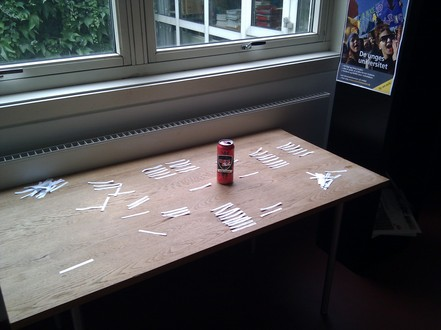
\includegraphics{affinitet/IMG_20100927_145008.jpg}
    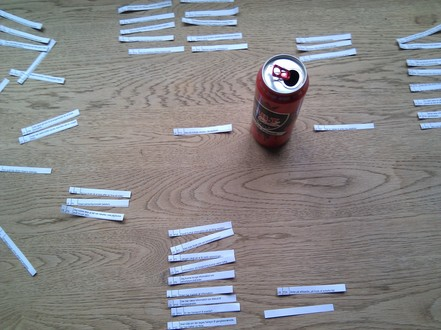
\includegraphics{affinitet/IMG_20100927_145025.jpg}
    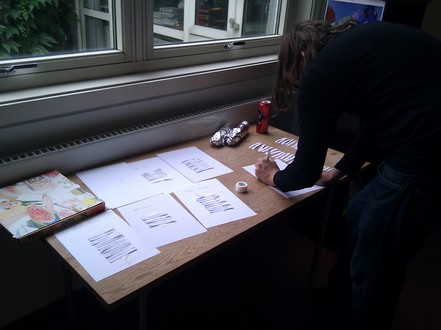
\includegraphics{affinitet/IMG_20100927_151239.jpg}
    \section{Visioner}
    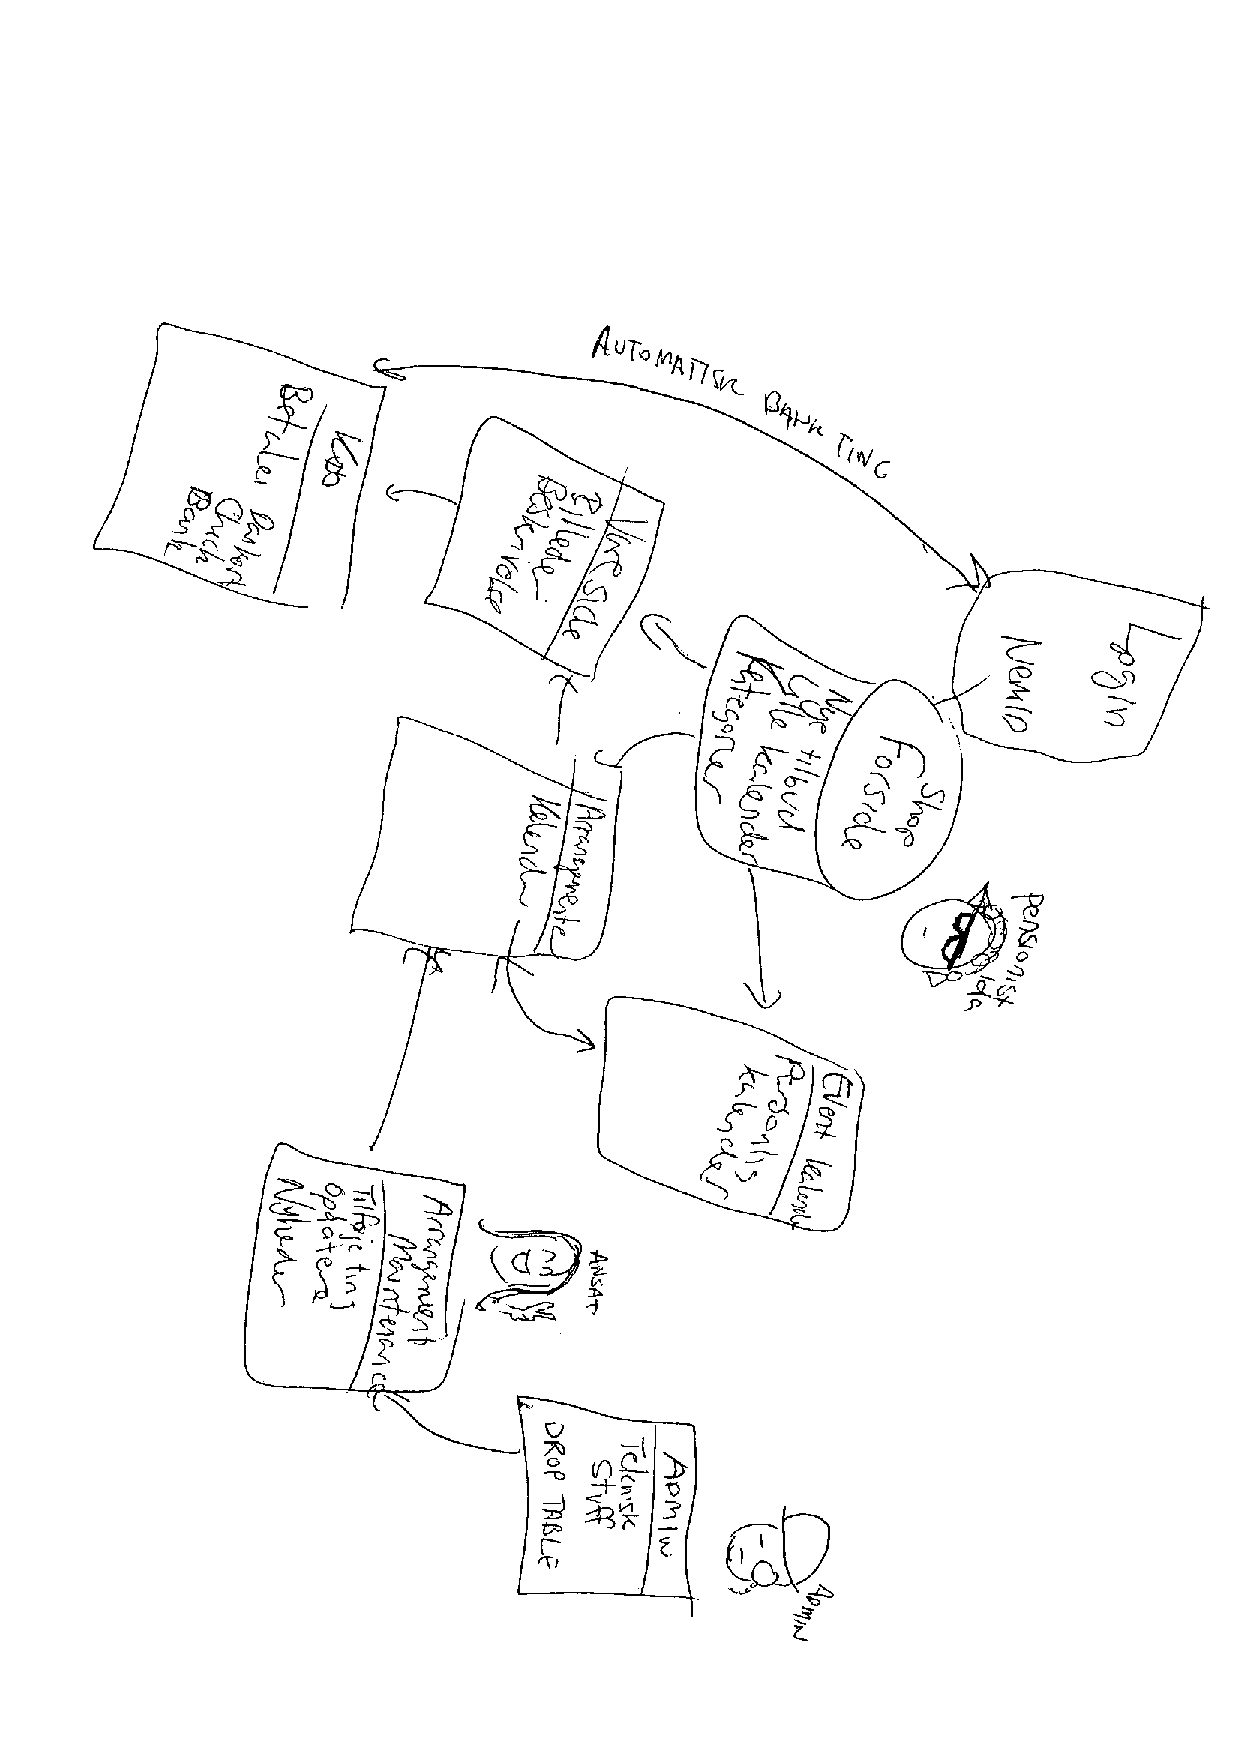
\includepdf[pages=-]{bilag_visioner.pdf}
    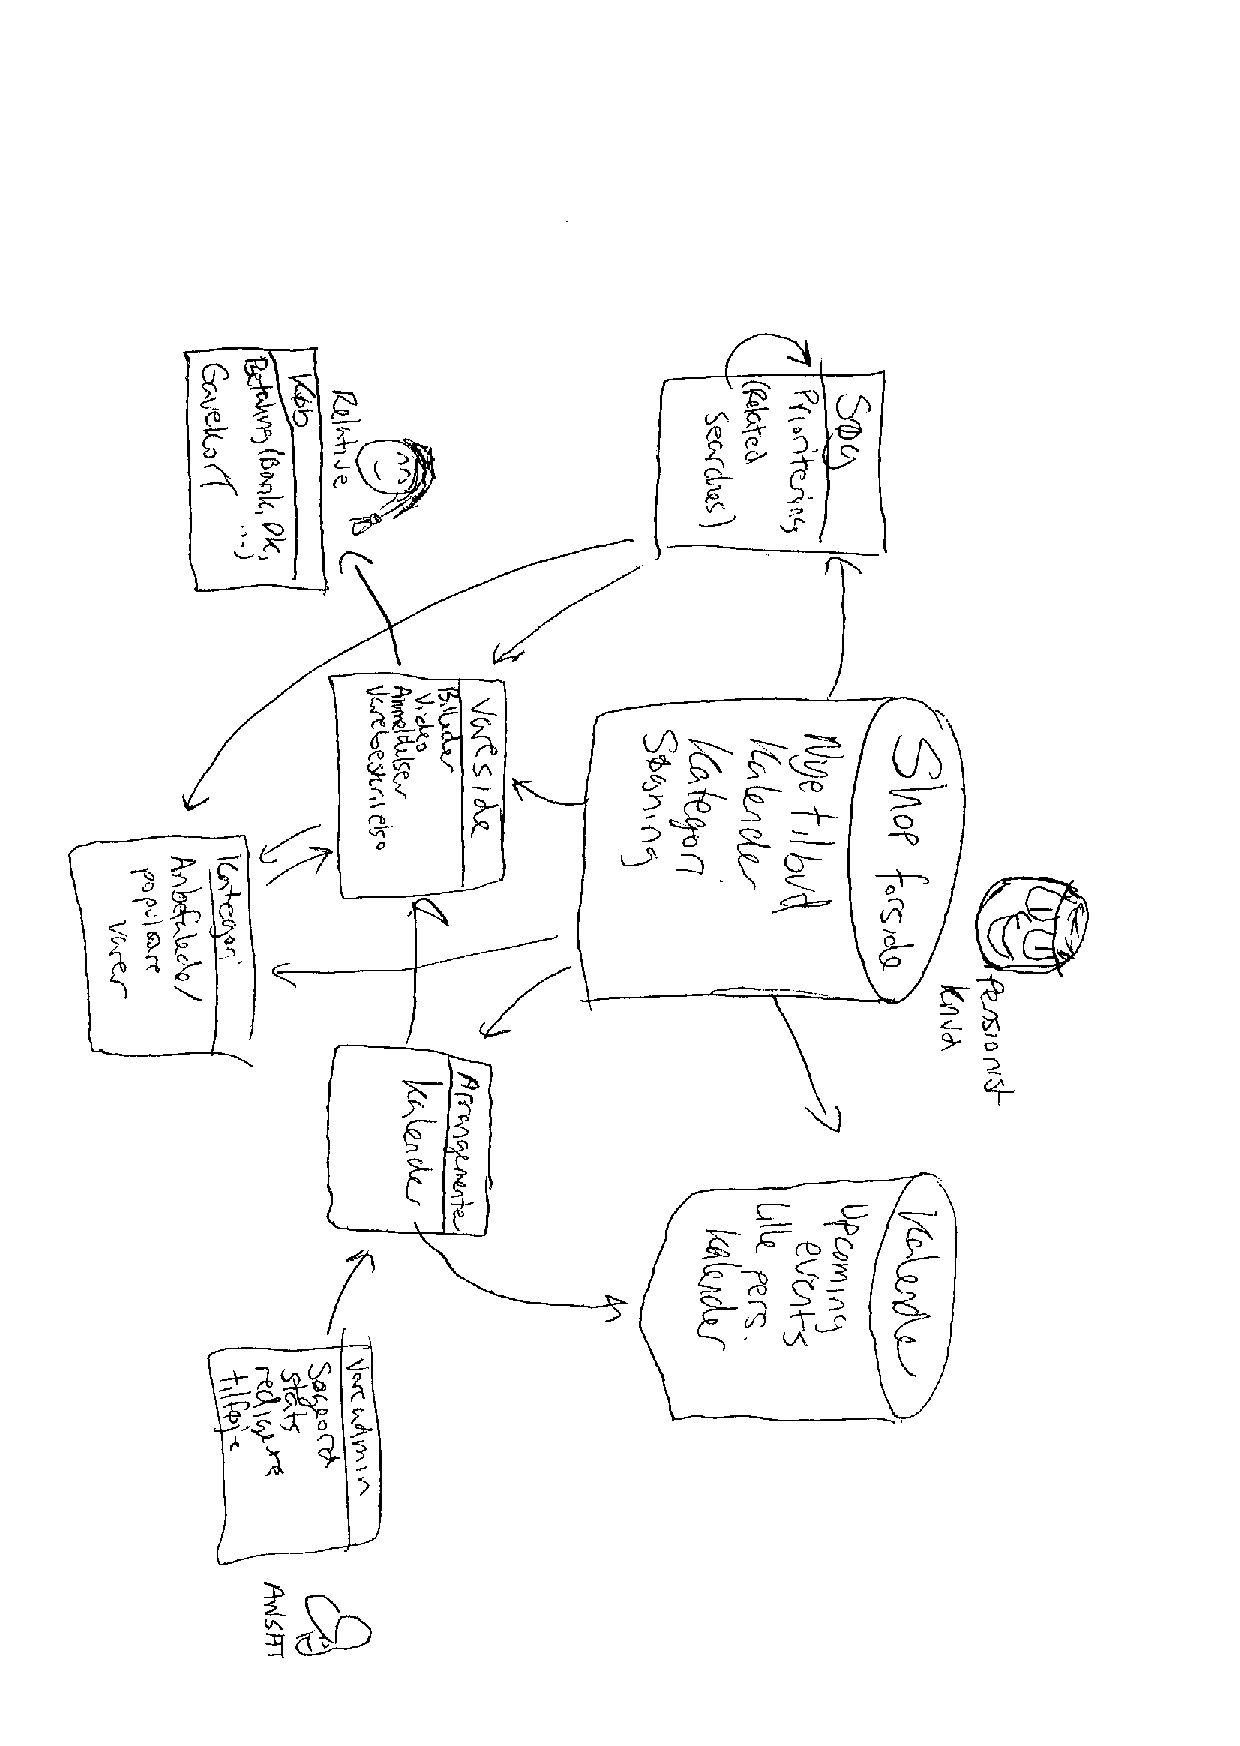
\includepdf[pages=-]{bilag_visioner_final.pdf}

    \section{Storyboards}
    
\includepdf[pages=2-3]{bilag_storyboards.pdf}
\end{appendices}

\end{document}
